\section{Symbôles sur lesquels faire de la médiation}
\label{section:simterpose}
Simterpose est l'API qui va nous permettre d'intercepter les communications de
l'application avec la machine sur laquelle elle s'exécute. Sans cela,
l'application se rendrait compte que l'environnement réel ne correspond pas
celui dans lequel elle pense s'exécuter.

\subsection{Organisation générale}
%schéma tableau
%\subsubsection{Interception des actions}
 Une application distribuée peut vouloir communiquer avec l'hôte soit pour
 effectuer de simples calculs (SEB), soit pour effectuer des requpetes de
 connexion ou de communication avec d'autres applications sur le réseau. Quand
 Simterpose intercepte une communication venant d'un des processus d'une
 application, il modifie les caractéristiques de cette dernière pour qu'elle
 puisse s'exécuter sur la machine hôte. Quand la machine hôte renvoie une
 réponse à l'application, Simterpose l'intercepte également et la modifie pour
 que l'application ne voit pas le changement d'architecture. En même temps, il
 envoie au simulateur des données concernant le temps d'exécution de l'action
 sur la machine hôte pour calculer le temps sur la machine simulée. Les délais
 calculés par le simulateur sont soit des temps de calculs soit des temps de
 connexion. Quand le simulateur à terminer le calcul du temps de réponse
 nécessaire il l'envoie à l'application en plus du résultat afin de mettre à
 jour l'horloge de l'appplication. Ainsi les calculs sont réellement exécuter
 sur la machine, les communications réellement émises sur le réseau géré par le
 simulateur et c'est le temps de réponse fourni par le simulateur qui va
 influencer l'horloge de l'application permettant ainsi d'imiter un
 environnement distribué. Finalement les applications ne communiquent plus
 directement entre elles puisque toute communication est interceptée par
 Simterpose puis gérée par le simulateur qui s'occupe du réseau.

{\color{red} Mettre deux schémas de action interceptes, test modifie, renvoie,
  attrape reponse, simulateur, retour application, un quand simple calcul l'autre quand conenxtion}

Pour intercepter ces actions, il faut d'abord choisir ce qu'on intercepte
exactement comme type d'action et avec quel outil. En effet une application peut
communiquer avec le noyau via différentes abstractions. Elle peut soit utiliser
les fonctions d'interraction directe avec le noyau que sont les appels systèmes,
soit utiliser les différentes abstractions fournies par le système
d'exploitation: bibliothèques (fonctions systèmes de la libc par exemple) ou les
fonctions POSIX dans le cas d'un système UNIX.

\begin{figure}[H]
 \centering
 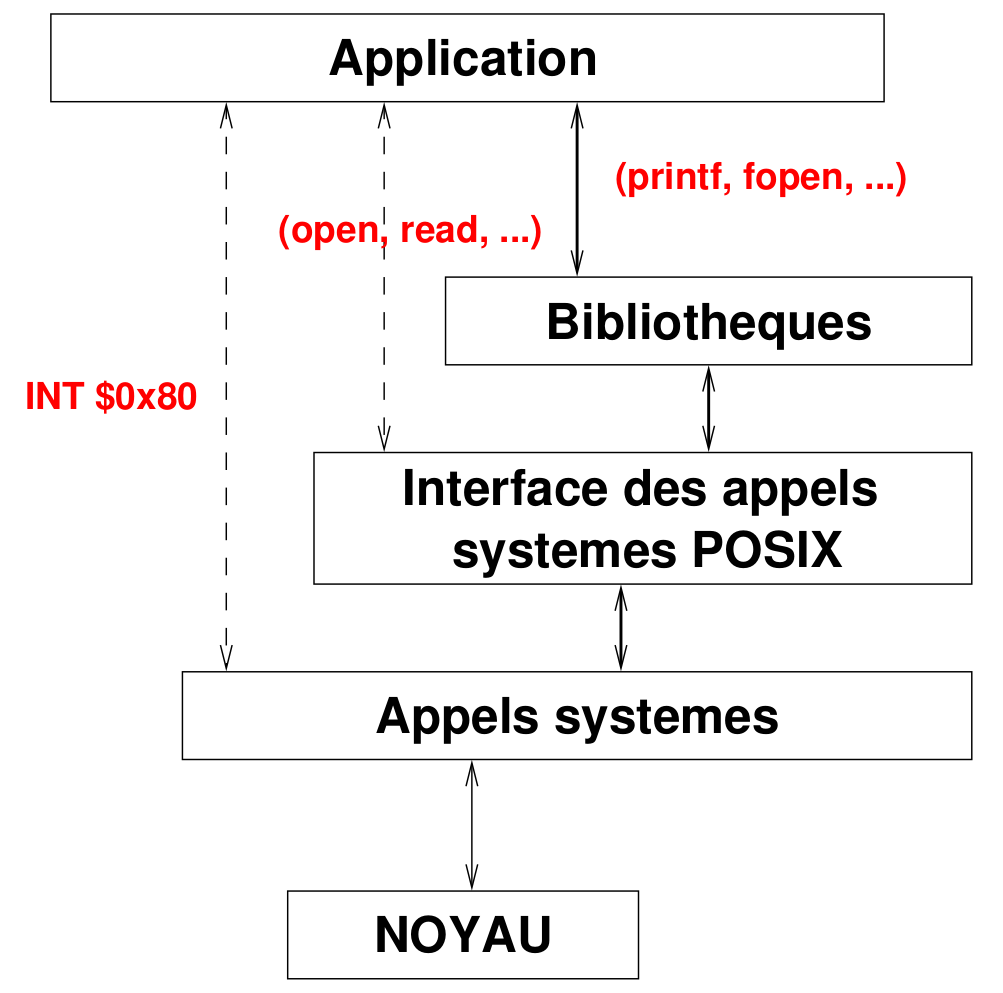
\includegraphics[scale=0.20]{Pictures/Communication_application_noyau.png}
 \caption{Communications possibles entre le noyau et une apllication}
 \label{AS_Communication}
\end{figure}

En regardant la Fig.\ref{AS_Communication}, et les différents niveaux d'abstractions, le plus simple pour attraper les actions de l'application en gérant un minimum de choses serait d'intercepter directement les appels systèmes. Nous allons donc voir comment il est possible de faire cela et si cette solution se suffit à elle même.

\subsection{Les communications réseaux}
 %-> syscall -> ptrace (full mediation, address translation)
Lorsque ptrace est appelé en entrée ou sortie d'appel système, les modifications
à apporter ne sont pas forcément les mêmes selon qu'il s'agit d'une action
nécessitant l'utilisation du réseau ou non. Dans le cas d'un simple calcul ce
qu'il faut maintenir pour l'application, c'est une vision du temps correspondant
à celle qui s'écoulerait si elle était vraiment sur la machine simulée. Ainsi en
entrée d'appel système on n'a pas besoin de modifier quoique ce soit, par contre
au retour il faut modifier le temps d'exécution du calcul en le remplaçant par
celui calculé par le simulateur. Dans le cas d'une communication réseau il faut
gérer la transition entre réseau local et réseau simulé. En effet l'application
possède une adresse IP et des numéros de ports ``virtuels'' qui ne correspondent
pas forcément à ceux attribués dans le réseau local. De plus on ne peut pas se
baser uniquement sur les numéros de \textit{file descriptor} associé à une
socket pour identifier deux entités qui communiquent entre elles.En effet ces
\textit{file descriptor} sont uniques pour chaque socket d'un processus, mais
plusieurs processus peuvent avoir un même numéro de \textit{file descriptor}
pour des sockets de communicatiosn différentes puisque chacune à son propre
espace mémoire. Pour pallier à ce probème on va utiliser en plus du numéro de
socket, les adresses IP et les ports locaux et distants des deux entités qui
souhaitent communiquer comme moyen d'identification. Pour gérer toutes ces
modifications deux solutions ont été proposées lors d'un précédent stage \cite{GUILLAUME:interception_syscall}: la
``médiation par traduction d'adresse'' et la ``full mediation''.

{\color{red}schéma}
\paragraph{Traduction d'adresse}
 Avec ce type de médiation on considère que le noyau gère des
 communications. Ainsi en entrée et sortie d'appel système Simterpose va juste
 s'occuper de la transition entre réseau ``virtuel'' et réseau local. Pour cela
 Simterpose gère un tableau de correspondance, dans lequel pour chaque
 application on a un couple (adresse IP et des ports ``virtuels'', adresse IP et
 ports ``réel'' sur le réseau).  De fait en entrée de l'appel système,
 Simterpose devra remplacer l'adresse et les ports ``virtuels'' de l'application
 par l'adresse et les ports réels sur le réseau local, ainsi l'appel système se
 fera avec une source qui existe réellement sur le réseau. Au retour de l'appel
 système il faudra remodifier les paramètres en remettant l'adresse et les ports
 ``virtuels'' pour que l'application pense toujours être dans son environnement
 simulé.  La limite de cette approche est lié au nombre de port disponibles sur
 l'hôte. 

\paragraph{Full mediation} 
Dans ce cas le noyau ne va plus gérer des communications car nous allons
empêcher l'application d'établir des connexions avec une autre application via
des sockets. Il n'y aura ni socket ni communication. Quand l'application voudra
faire un appel système de type communication vers une autre applciation, le
processus espion de Simterpose qui sera notifié via ptrace neutralisera l'appel
système. Ensuite ce processus en utilisant ptrace récupérera en lisant dans la
mémoire du processus espionné les ifnormations à envoyer ou récupérer et ira
directement lire ou écrire ces informations dans la mémoire du
destinataire. Ainsi on n'a pas besoin de gérer de tableau de correspondance
d'adresse et de ports et les applications peuvent conserver les adresses
simulées qu'elles considèrent comme réelles.  Même si la ``full mediation''
permet d'éviter les communications réseaux et de conserver des tables de
correspondances, dans le cas d'applications qui communiquent énormément et
utilisent de grosses données elle s'avère moins efficace. En effet les appels à
mémoires sont bien plus couteux que les communications réseaux.

\subsection{Les thread}
 syscall clone + libcalls

\subsection{Le temps}
 -> syscall (- system wide), VDSO-linker (cross process ou VDSO)

\subsection{DNS}
libcalls (ne rien rater), config fake (system wide), intercept 53 ( plus dur que nécessaire, port dns autre ou pas)
